\section{The Middle Pillar}

\paragraph{The Three Pillars}

\begin{wrapfigure}{rt}{.3\textwidth}
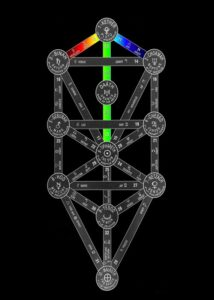
\includegraphics[width=.25\textwidth]{MiddlePillar-214x300.jpg}
\end{wrapfigure}

The three pillars of the Cabala Tree of Life represent the process of manifestation from God to the World, and also the path back. On the principle that the microcosm reflects the macrocosm, the Tree of Life also refers to our inner structure.

The right pillar is masculine and the left pillar is feminine. The middle pillar, then, is the reconciling force, as it synthesizes the right and left paths. In the Meditations on the Tarot, Valentin Tomberg refers to four syntheses, represented by the Sephiroth on the Middle Pillar:

\begin{itemize}


\item \textbf{Malkuth} is the synthesis the entire paths in the world of action

\item \textbf{Yesod} is the synthesis of romantic love between the sexes

\item \textbf{Tiphareth} is the synthesis revealed through artistic creativity

\item \textbf{Daath} is the synthesis of Intelligence and Wisdom in the act of knowledge, or gnosis
\end{itemize}


\paragraph{Daath and Kether}


\begin{wrapfigure}{rt}{.3\textwidth}
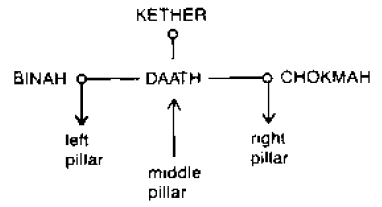
\includegraphics[width=.25\textwidth]{daath.png}
\end{wrapfigure}

Daath is a crypto-sephirah, that is, it is not one of the 10 sephiroth. That is because it is not given to us by natural birth, but is something that must be created in a second birth. It arises via the synthesis of Intelligence and Wisdom. Tomberg defines it this way:

\begin{quotex}
Daath is therefore the state of consciousness where intelligence and wisdom --- acquired and acquirable knowledge, on the one hand, and latent and actualisable knowledge, on the other hand --- become one.
\end{quotex}

Since Daath is the image of Kether, they should not both be represented in the Tree together. Either one or the other is shown. This means that the Sephiroth of Binah and Chokmah, when Kether is omitted, both derive from Daath, as shown in this diagram.

\paragraph{Intelligence}


Intelligence is knowledge we acquire about the world. That is why it is feminine, or lunar. It does not provide its own light, but can only reflect on things. Regarding the higher things, it is capable of understanding God as the Absolute and the Infinite, even if those terms are commonly misunderstood. For example, the Infinity of God is often interpreted in mathematical terms, which leads to incorrect ideas.

Through natural intelligence, God can also be known as the First Cause, Unmoved Mover, etc. However, God cannot be known as Spirit, as an ``I''. For that, it must be illumined through a spiritual marriage with Wisdom. Our feminine age is overly intellectual and rejects the other ways of knowing that are revealed in the Cabala.

\paragraph{Wisdom}


Wisdom represents knowledge that is latent or virtual, and it must be actualized. Man is not a \emph{tabula rasa}, and is not as malleable as those on the left hand path would like. There is instinctual knowledge, as \textbf{Henri Bergson} points out, that needs to rise to the level of intelligence. There is a nagging forgetfulness, both horizontal and vertical, that must be brought up into the light of consciousness. This vague memory of a different world is what drives the religious impulse. Whatever might seem absurd to natural Intelligence, is actually a natural challenge to the presumed and hubristic superiority of Intelligence. In \emph{The Two Sources of Morality and Religion}, Bergson explains:

\begin{quotex}
Since instinct no longer exists except as a mere vestige or virtuality, since it is not strong enough to incite to action or prevent it, it must arouse an illusory perception, or at least a counterfeit of recollection so clear and striking that intelligence will come to a decision accordingly. ... \emph{religion is then a defensive reaction of nature against the dissolvent power of intelligence.}
\end{quotex}


At its best, religion will force the Intelligence out of its box in order to confront something higher. In the synthesis with Wisdom, Tomberg says:

\begin{quotex}
the intelligence unites with and understands things that it would never have understood from within itself. It is therefore ``illumined''.
\end{quotex}


At its worst, this defensive reaction of the instincts may devolve into superstitions and illusions. Practices arise with the aim of producing mere sensory phenomena, which are then misconstrued as spiritual enlightenment. Of course, certain phenomena may arise as side effects, as we see in some saints, but they should never be the primary aim. Tomberg points out that breathing exercises, postures, etc. cannot, on their own, lead to inspiration.

\paragraph{Direction of the Middle Pillar}


\begin{wrapfigure}{rt}{.3\textwidth}
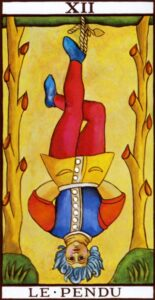
\includegraphics[width=.25\textwidth]{major12-155x300.jpg}
\end{wrapfigure}

The directions of the paths of the left and right pillars of the Cabala are downward, whereas that of the middle pillar is upward. The left and right pillars bring divine governance down to the world. Then the synthesis of the two paths results on Malkuth, or the Kingdom. Between the sephiroth of Kether (the Crown) and Malkuth (the Kingdom), there are three levels that represent the soul activities of thinking, feeling, and willing. In the Letter on the \textbf{Hanged Man}, we read:

\begin{quotex}
The normal relationship between thought, feeling and the will for a civilised and educated man is such that his thought awakens feeling and directs the will. Thought plays a stimulating role, by means of imagination, towards feeling, and an educative role, by means of imagination and feeling, towards the will. Having to act, one thinks, one imagines, one feels, and lastly, one desires and acts.
\end{quotex}


So, on the left pillar, the organ of thought is the Intellect and on the right, the organ of thought is Revelation. However, looking at the Middle pillar, the place that thought should occupy --- namely Daath --- is missing. Hence, it cannot be the beginning of the path, but rather the terminus. This is represented by the Hanged Man, where we read this explanation:

\begin{quotex}
For the ``spiritual man'' it is the will which plays the stimulating and educative role towards feeling and thought. He acts first, then he desires, then he feels the worth of his action, and lastly he understands.
\end{quotex}


This means that on the Middle Path, the return to God, the spiritual man must act first before he fully understands. On the upward path, Will changes from ``my will'' to ``thy will'' be done. The will begins in obedience. Ultimately, the path leads to Daath, intuition, gnosis. Here we see the truth of \textbf{St Augustine}'s saying:

\textit{crede, ut intelligas}


\flrightit{Posted on 2022-05-19 by Cologero}

\begin{center}* * *\end{center}

\begin{footnotesize}
\begin{sffamily}
\texttt{Balder on 2022-05-20 at 13:59 said:}

As the hanged man sees it, it is the world that is upside down.

\hfill

\texttt{Michael DeJoy on 2022-05-22 at 22:27 said:}

Cologero, recently I have been wondering whether every person who dies enters a post mortem state and goes on to higher levels or it may be that not everyone who dies actually survives in a post mortem realm and rather may just have their consciousness disappated over time. If a man does not make spiritual efforts as mentioned in the article then there may be no reason or necessity for continued survival. Many people have no clue as to what they should do to raise consciousness and without that I don't see what the future will hold for them.

\hfill

\texttt{Cologero on 2022-05-22 at 23:31 said:}

That is a great question, Michael. Keep in mind that the esoteric path is for a few. Those who are called must follow it, but that does not make it superior to those who follow the exoteric path; they make efforts their own way. As for those who follow neither, I don't see what the future holds for them either; but I can't judge. Although the animal soul is still material, it is not eternal. But he rational soul is life which cannot end, yet it is just a state of something higher.

If you want to ponder something, watch the last 10 minutes or so of this: \textit{Zoe's Story}\footnote{\url{https://www.youtube.com/watch?v=rqSmm_gYsvk}}. We don't have, and never will, a rational answer to everything.

\end{sffamily}
\end{footnotesize}

